\chapter{Compile and run MPI programs}

As expected, running the unmodified hello program results in several \textit{Hello World!} being printer, one for each processor we are running on.

After modification of the program, we have the following result:
\begin{figure}[!h]
\begin{center}
	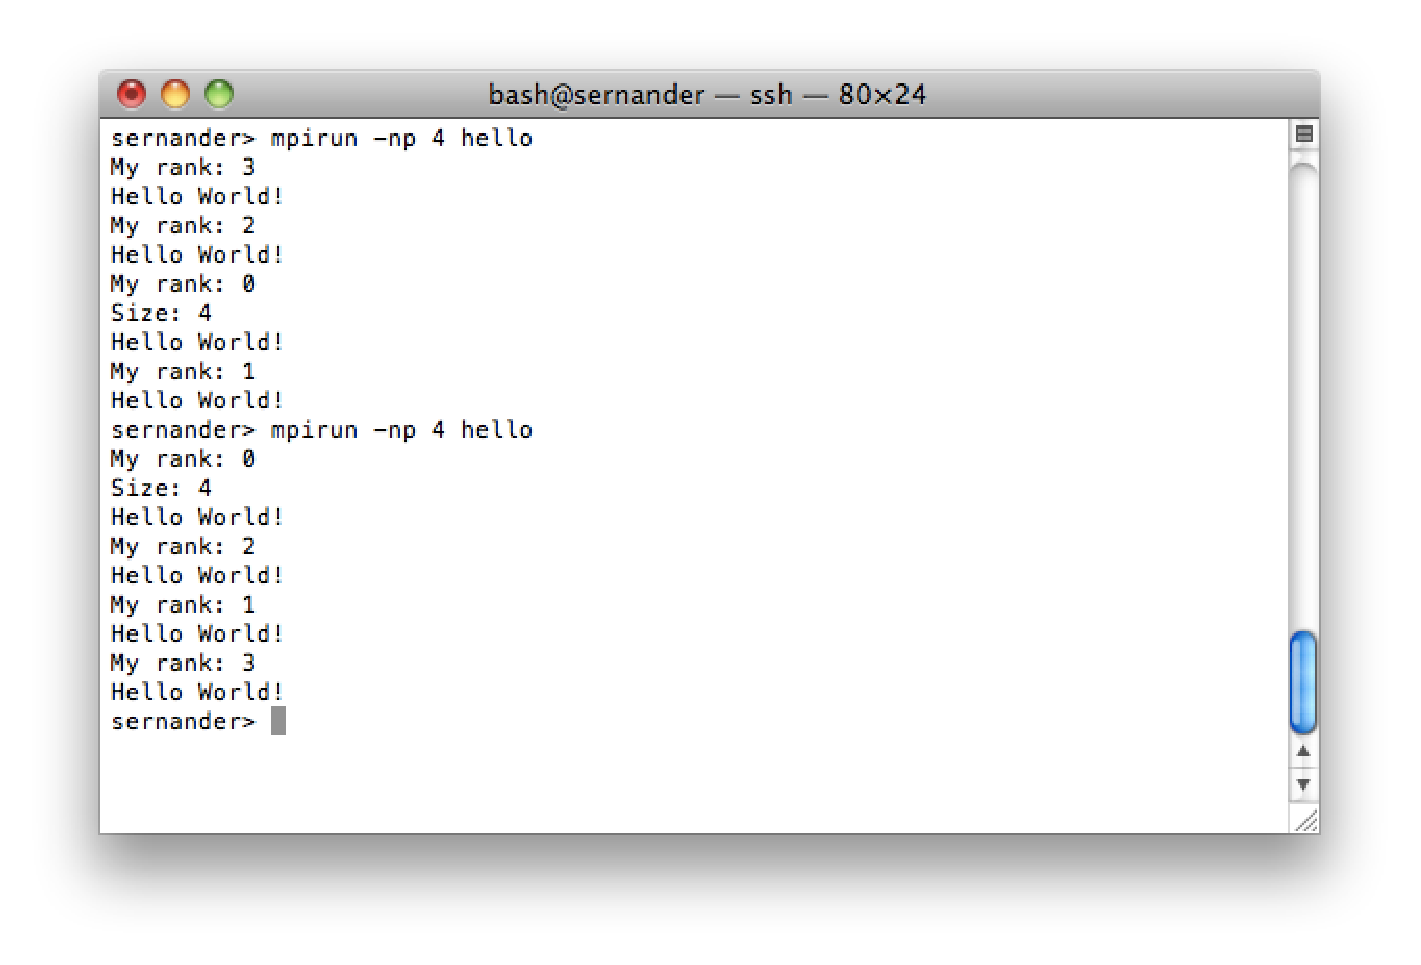
\includegraphics[width=\textwidth]{pic/hello.eps}
	\caption{Result of the modified hello program}
\end{center}
\end{figure}

We can see that only the processor with rank 0 prints the number of processors. The picture also shows that there is no pre-defined order between the processors because the order of the messages changes. This is normal because the processes created are scheduled independly on their processor. So, there is no way to tell which one will start first or in which order the result will appear.

